%!LW recipe=pdflatex

\documentclass{standalone}

\usepackage{animate}
\usepackage{amsmath, amssymb, amsthm, mathrsfs, amsfonts, dsfont}
\usepackage{ascmac}
\usepackage{bbm}
\usepackage{bm}
\usepackage{breakcites}
\usepackage{calc}
\usepackage[style=base]{caption}
\usepackage{enumerate}
\usepackage[T1]{fontenc}
\usepackage{ifthen}
\usepackage{mathtools}
\usepackage{makecell}
\usepackage{mlmodern}
\usepackage{newtxtext}
\usepackage{optidef}
\usepackage{physics}
\usepackage{pifont}
\usepackage{setspace}
\usepackage{stfloats}
\usepackage{subcaption}
\usepackage{svg}
\usepackage{tikz}
\usepackage{xparse}
\usepackage[all]{xy}

\usepackage{float}
\usepackage{color}
\usepackage{graphicx}
\usepackage[colorlinks=true, allcolors=blue]{hyperref}


% === Commands ===

\definecolor{cA}{HTML}{0072BD}
\definecolor{cB}{HTML}{EDB120}
\definecolor{cC}{HTML}{77AC30}
\definecolor{cD}{HTML}{D95319}
\definecolor{cE}{HTML}{7E2F8E}
\newcommand{\cAText}[1]{\textcolor{cA}{#1}}
\newcommand{\cBText}[1]{\textcolor{cB}{#1}}
\newcommand{\cCText}[1]{\textcolor{cC}{#1}}
\newcommand{\cDText}[1]{\textcolor{cD}{#1}}
\newcommand{\cEText}[1]{\textcolor{cE}{#1}}
\newcommand{\red}[1]{\textcolor{red}{#1}}
\newcommand{\blue}[1]{\textcolor{blue}{#1}}
\newcommand{\green}[1]{\textcolor{green}{#1}}
\newcommand{\gray}[1]{\textcolor{gray}{#1}}
\newcommand{\black}[1]{\textcolor{black}{#1}}

\usetikzlibrary{
  3d,
  fit,
  calc,
  math,
  matrix,
  patterns,
  backgrounds,
  arrows.meta,
  decorations.pathmorphing,
}

\begin{document}
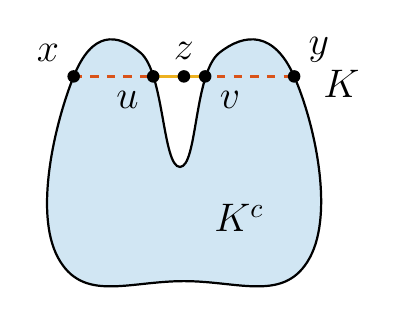
\begin{tikzpicture}[
    scale=1,
    K/.style={thick, draw=black, fill=cA!18},
    crosscut/.style={very thick, draw=cB},
    noncrosscut/.style={very thick, draw=cD, dashed},
    pt/.style={circle, fill=black, inner sep=1.6pt},
    lab/.style={font=\Large},
    note/.style={font=\Large, align=center}
]

% ============================================================
% Example 3: not a crosscut
% x,y are exactly vertices on bd K.
% The open segment leaves K through the indentation.
% ============================================================
\begin{scope}[shift={(10.0,0)}]
    \coordinate (A3) at (0.0,0.3);
    \coordinate (x3) at (0.2,2.6);
    \coordinate (B3) at (1.05,2.9);
    \coordinate (C3) at (1.55,1.45);
    \coordinate (D3) at (2.05,2.9);
    \coordinate (y3) at (3.0,2.6);
    \coordinate (E3) at (3.2,0.3);
    \coordinate (F3) at (1.6,0.0);

    \draw[K]
        plot[smooth cycle, tension=0.8] coordinates {
            (A3) (x3) (B3) (C3) (D3) (y3) (E3) (F3)
        };

    % Define intermediate points
    \coordinate (z3) at (1.6,2.6);
    \coordinate (u3) at (1.21,2.6);
    \coordinate (v3) at (1.87,2.6);

    \draw[noncrosscut] (x3) -- (z3);
    \draw[noncrosscut] (z3) -- (y3);
    \draw[crosscut] (u3) -- (v3);

    \node[pt,label={[lab]above left:$x$}] at (x3) {};
    \node[pt,label={[lab]above right:$y$}] at (y3) {};
    \node[pt,label={[lab]above:$z$}] at (z3) {};
    \node[pt,label={[lab]below left:$u$}] at (u3) {};
    \node[pt,label={[lab]below right:$v$}] at (v3) {};

    % Region labels
    \node[lab] at (2.3,0.8) {$K^c$};
    \node[lab] at (3.6,2.5) {$K$};
\end{scope}

\end{tikzpicture}
\end{document}
